\section{Evaluation}\label{sec:evaluation}

The current artifact contains completed runs for three format-parser pairs: URI with Curl, JSON with json-c, and ELF with libelf.
Manual per-block review is complete for ELF; URI and JSON results are descriptive counts from the committed outputs.
Apache APR and HPACK are retained as planned extensions, not completed evaluations.

\textbf{Research questions.}
\begin{itemize}
    \item[\textbf{(Q1)}] How many basic blocks does \toolname label, and what fraction of the trace-derived graph do those labels cover?
    \item[\textbf{(Q2)}] For the reviewed ELF output, how accurate are the labels at the per-block level?
    \item[\textbf{(Q3)}] What preliminary differences appear across the three completed format-parser runs?
\end{itemize}

\subsection{Methodology}\label{sec:eval:method}

For each completed format-parser pair, we (1)~compile a harness against the parser library inside a Docker container with debug symbols and static linkage, and (2)~run \toolname with the corresponding grammar template under \QEMU user-mode.
For ELF, a human evaluator additionally checks each production-labeled block against the source location recovered via \texttt{addr2line} and classifies it as a strict true positive, false positive, or marginal case.
Because the evaluation does not enumerate all semantically relevant parser blocks independently of \toolname, it does not measure false negatives.

\textbf{Why manual inspection.}
Automated semantic verification without ground truth can introduce circularity or unsupported judgments.
Accordingly, the ELF accuracy result comes from manual inspection of the labeled graph, source mappings, and relevant parser routines.
URI and JSON accuracy values are intentionally left unreported until the same review is complete.

\subsection{URI Parsers}\label{sec:eval:url}

The completed URI run targets Curl's \texttt{curl\_url\_set}; a run against Apache Portable Runtime's \texttt{apr\_uri\_parse} remains planned.
The URI template instantiates 1{,}458 inputs and produces 2{,}124{,}306 ordered comparisons between distinct inputs.

\textbf{Curl.}
On the statically linked Curl harness, \toolname produces a trace-derived graph with 522 nodes and 558 edges.
The committed mapping contains 191 production-labeled blocks across 10 exact label strings and 21 blocks with the ambiguous \texttt{None} label.
Table~\ref{tab:url-labels} shows the distribution.
Host validation dominates because Curl's parser performs extensive checks: IPv4 versus IPv6 detection, IDNA processing, bracket handling, and length validation.
The duplicate-looking labels (\texttt{port} versus \texttt{:port}, \texttt{query} versus \texttt{?query}) come from the template's leaf naming: the colon or question mark delimiter is included in the label string. This is a template quirk; the underlying attribution is correct.

\begin{table}[h]
\caption{URI label distribution (Curl).}
\label{tab:url-labels}
\centering
\begin{tabular}{lr}
\toprule
Production & Labeled BBs \\
\midrule
host        & 91 \\
port        & 34 \\
segment     & 30 \\
userinfo    & 25 \\
query       & 5  \\
fragment    & 5  \\
path        & 1  \\
\textit{ambiguous} & 21 \\
\bottomrule
\end{tabular}
\end{table}

The 21 ambiguous blocks are code paths that the current filtering could not uniquely attribute to a single production.
Per-block accuracy has not yet been reviewed.

\textbf{Apache APR.}
The repository documents this as a planned replication with the same URI template, but it contains no APR output from which to report results.

\subsection{JSON Parsers}\label{sec:eval:json}

We evaluate on json-c, a widely deployed C library for JSON parsing.
The JSON template instantiates 27 inputs and produces 702 ordered comparisons between distinct inputs.

On json-c (commit \texttt{894856}), \toolname produces a trace-derived graph with 464 nodes and 400 edges, of which 295 basic blocks receive production labels across 6 productions.
Table~\ref{tab:json-labels} shows the distribution.

\begin{table}[h]
\caption{JSON label distribution (json-c).}
\label{tab:json-labels}
\centering
\begin{tabular}{lr}
\toprule
Production & Labeled BBs \\
\midrule
number         & 110 \\
object-element & 77  \\
string         & 39  \\
array          & 36  \\
boolean        & 24  \\
nan            & 9   \\
\bottomrule
\end{tabular}
\end{table}

\texttt{number} dominates because C-level numeric parsing is complex: sign handling, decimal point, exponent notation, overflow checks, and \texttt{strtod} wrappers each require their own basic blocks.
\texttt{nan} receives few labels because the parsing path is a three-character string comparison.

Per-block accuracy has not yet been reviewed for this output.

\subsection{HPACK Decoder}\label{sec:eval:hpack}

HPACK is the header compression format for HTTP/2, defined in RFC~7541~\cite{rfc7541}.
The format is fully binary, uses context-sensitive encoding, and includes a fixed Huffman table baked into the specification.
This would make HPACK a useful stress test for \toolname: it has binary encodings and conditional logic that text formats lack.
The planned target is nghttp2's HPACK decoder, but the repository does not yet contain a template or output for this evaluation.

\subsection{ELF Parser}\label{sec:eval:elf}

ELF is the standard binary format on Linux and other Unix-like systems.
Unlike the sequential text formats above, ELF is offset-driven: the ELF header contains pointers to program header and section header tables, which in turn point to string tables, symbol tables, and other sections.
We target libelf from elfutils, a widely used library for accessing ELF files.

\textbf{Corpus layout.}
Figure~\ref{fig:elf-layout} shows the layout of a single corpus instantiation.
Every corpus member is exactly 1{,}048 bytes with identical offsets, and varies only in three regions: the ELF header (one variant), the two-entry program header table (four variants that change the second program header's type field across \texttt{PT\_NOTE}, \texttt{PT\_INTERP}, \texttt{PT\_DYNAMIC}, and \texttt{PT\_NULL}), and the section region (five variants that toggle which sections contain real data versus zeroed bytes).
The Cartesian product yields $1 \times 4 \times 5 = 20$ instantiations and 380 pairwise comparisons.

\begin{figure}[t]
\centering
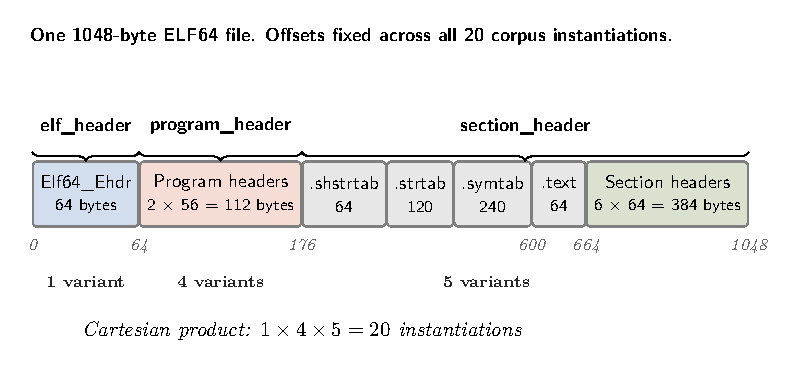
\includegraphics[width=\linewidth]{figures/elf-layout.pdf}
\caption{Fixed-layout ELF corpus. Every one of the 20 instantiations has the same byte offsets. The three template children (\texttt{elf\_header}, \texttt{program\_header}, \texttt{section\_header}) carry 1, 4, and 5 alternatives respectively.}
\label{fig:elf-layout}
\end{figure}

\textbf{Results.}
On libelf, \toolname produces a labeled trace-derived graph with 358 nodes and 354 record-pair edges.
Of these, 68 basic blocks receive the \texttt{section\_header} label.
The \texttt{program\_header} production receives zero labels despite having four template variants.

\textbf{Why \texttt{program\_header} is unlabeled.}
Libelf reads all program-header types through the same code path.
The \texttt{p\_type} field is data stored in a struct; libelf does not branch on it during parsing.
The retained translation-log evidence through \texttt{gelf\_getphdr} is therefore identical across the four variants, and the difference algorithm has no record pairs to attribute.
Section types, by contrast, do trigger different code paths: sections with \texttt{SHT\_SYMTAB} type cause the harness to iterate symbol entries via \texttt{gelf\_getsym} and resolve names via \texttt{elf\_strptr}, while null sections skip these operations.

\begin{table}[h]
\caption{ELF label distribution (libelf). The high ambiguity rate reflects libelf's structure: most code is shared across section types.}
\label{tab:elf-labels}
\centering
\begin{tabular}{lr}
\toprule
Production & Labeled BBs \\
\midrule
section\_header & 68 \\
\textit{ambiguous} & 202 \\
\bottomrule
\end{tabular}
\end{table}

\textbf{Where the labels land.}
Figure~\ref{fig:elf-cfg} shows 12 of the 68 labeled blocks, taken directly from our \texttt{out.dot}.
They cluster in three places: the harness's \texttt{walk\_section\_headers} loop, libelf's \texttt{\_\_libelf\_set\_rawdata\_wrlock} section-data initialization routine, and libelf's lookup routines (\texttt{elf\_strptr}, \texttt{gelf\_getsym}).
The cross-function arrows are consecutive records in the QEMU translation log: the corresponding paths appear when the harness reaches libelf's section setup and symbol-table walk for sections that carry a symbol table.

\begin{figure}[t]
\centering
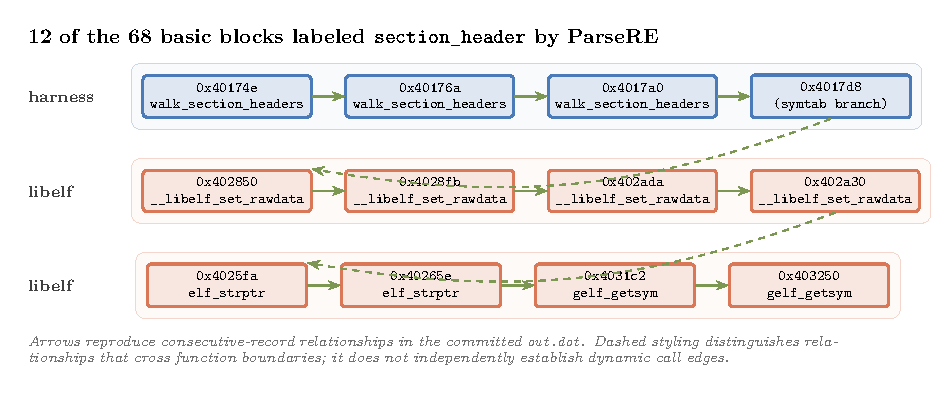
\includegraphics[width=\linewidth]{figures/elf-cfg-fragment.pdf}
\caption{12 of the 68 \texttt{section\_header}-labeled basic blocks. Arrows reproduce consecutive-record relationships from the committed trace-derived graph; dashed styling distinguishes relationships that cross function boundaries.}
\label{fig:elf-cfg}
\end{figure}

\textbf{Accuracy.}
Manual inspection of all 68 labeled blocks yields 62 strict true positives (91.2\%), 5 false positives, and 1 marginal case.
The 5 false positives all sit inside \texttt{\_\_gelf\_getehdr\_rdlock}, an ELF-header validation routine that libelf calls internally during section traversal.
Those blocks process the ELF header rather than section headers, but they are reached only through section-handling code paths and so appear in the differential edge set.
The review did not measure false negatives because it did not independently enumerate every block that should receive a grammar label.

\textbf{What this reveals about binary formats.}
The text-format runs produce 6 JSON label strings and 10 exact URI label strings, while the ELF run produces one (\texttt{section\_header}).
This result is consistent with the tested libelf harness using uniform record readers for many structures and conditional consumer code for section and symbol-table handling.
It should not yet be generalized to binary parsers as a class from one evaluated target.

\subsection{Cross-Format Comparison}\label{sec:eval:comparison}

\begin{table}[t]
\caption{Cross-format artifact summary. Inst.\ = template instantiations; BBs = total blocks in the trace-derived graph; Labels = production-labeled blocks; Acc.\ = strict true positives divided by all production-labeled blocks.}
\label{tab:crossformat}
\centering
\begin{tabular}{llrrrr}
\toprule
Format & Parser & Inst. & BBs & Labels & Acc.(\%) \\
\midrule
URI    & Curl          & 1{,}458  & 522  & 191  & -- \\
URI    & Apache APR    & 1{,}458  & --   & --   & -- \\
JSON   & json-c        & 27       & 464  & 295  & -- \\
HPACK  & nghttp2       & --       & --   & --   & -- \\
ELF    & libelf        & 20       & 358  & 68   & 91.2 \\
\bottomrule
\end{tabular}
\end{table}

\textbf{Coverage is not a function of corpus size.}
JSON uses 27 instantiations and labels 295 blocks (63.6\% of the graph).
URI uses 1{,}458 instantiations and labels 191 blocks (36.6\%), with 21 additional ambiguous records.
ELF uses 20 instantiations and labels 68 blocks (19\%).
These three observations show that a larger corpus does not automatically yield a higher labeling rate.
More formats, parsers, and reviewed outputs are required before attributing the differences to a format class or parser architecture.
